\documentclass[a4paper,11pt]{article}
\usepackage[T1]{fontenc}
\usepackage[utf8]{inputenc}
\usepackage{lmodern}
\usepackage{ngerman}
\usepackage{amsmath}
\usepackage{graphicx}

\setcounter{secnumdepth}{0}
\title{Übungsblatt 01}
\author{Lennard Behrens, Tizian Roth}

\begin{document}

\maketitle

\section{Aufgabe 1}

Da aus den Messungen nicht hervorgeht, welches Photon des Laserpulses vom Detektor gemessen wird, folgt die Messungenauigkeit aus der Sensorauflösung. Zudem muss beachtet werden, dass gilt $2\Delta s$, da der Laserimpuls zum Mond hin und wieder zurück läuft.
Für die absolute Messungenauigkeit gilt dann folglich \\
\begin{center}
  $\Delta s = \frac{1}{2} T \cdot c = \frac{1}{2} 1,50 \cdot 10^{-10} \mbox s \cdot 3,0 \cdot 10^{8} \mbox{m/s} = 2,25 \mbox{cm}$ .
\end{center}
Wobei $T$ der zeitliche Abstand zwischen den Messungen und $c$ die Lichtgeschwindigkeit ist. \par
Für die relative Messungenauigkeit gilt dann
\begin{center}
  $\frac{2\Delta s}{s} = 3,4 \cdot 10^{-10} $ .
\end{center}


\section{Aufgabe 2}

Aus dem vorgegebenen Faktor folgt für die relative Zeitabweichung
\begin{center}
  $\frac{\Delta t}{t} = 1 - \sqrt{1 - \frac{v^2}{c^2}}$ .
\end{center}
Aus Erfahrung weiß man, dass eine Fahrt von Marburg nach Gießen und zurück etwa $30$ Minuten dauert. 
Für die Geschwindigkeit des Zuges gilt die grobe Näherung
\begin{center}
  $v = \frac 1 3 \cdot 10^2 \mbox{m/s}$ .
\end{center}
Daraus ergibt sich dann die relative Zeitabweichung von
\begin{center}
  $\frac{\Delta t}{t} = 6,2 \cdot 10^{-15} $
\end{center}
und eine absolute Zeitabweichung von
\begin{center}
  $\Delta t = 1800 \mbox{s} \cdot 6,2 \cdot 10^{-15} = 11 \mbox{ps}$ .  
\end{center}


\section{Aufgabe 3}

\subsection{Aufgabe 3a}
Für die Zeit, die das Licht von Beteigeuze zur Erde braucht, gilt 
\begin{center}
  $\Delta t = \frac{d}{c} = \frac{6,0 \cdot 10^{18}\mbox{m}}{3,0 \cdot 10^8 \mbox{m/s}} = 634\mbox{a}$ .
\end{center}

\subsection{Aufgabe 3b}
Für die Entfernung in Abhängigkeit zu $\delta$ gilt
\begin{center}
  $
    \sin \delta = \frac{r}{d} \Leftrightarrow 
    \delta     = \arcsin\frac{r}{d} = 2,5 \cdot 10^{-8}
  $
\end{center}
Wobei $r$ der Abstand zwischen Erde und Sonne ist.

\subsection{Aufgabe 3c}
Für die Entfernung zum Stern gilt der Zusammenhang
\begin{align*}
  d = \frac{r}{\sin \delta} \mbox{.}
\end{align*}
Nun weicht die Messung der Sternparallaxe um $\pm\Delta\delta$ von der tatsächlichen Entfernung ab. Wodurch sich eine absolute Messungenauigkeit $\pm\Delta d$ ergibt. Da sich bei so kleinen Winkeln der $\sin \delta$ verhält, gilt für die absolute Messungenauigkeit
\begin{align*}
  \Delta d = \frac{r}{\sin\delta } \mbox{.}
\end{align*}
Da der Winkel $\delta$ sehr klein ist, gilt folgende Näherung
\begin{align*}
  d = \frac{r}{\delta} \mbox{.}
\end{align*}
Da $d$ nichtlinear abhängig von $\delta$ ist, schätzt man den Fehler mithilfe der Ableitung ab. Solange $\Delta\delta \ll \delta$ ist, gilt
\begin{align*}
  \frac{d}{d \delta} d &= -\frac{r}{\delta^{2}} \mbox{.}
\end{align*}
Die Ableitung kann dann wie folgt genähert werden
\begin{align*}
  \frac{d}{d \delta} d \approx \frac{\Delta d}{\Delta \delta} \Rightarrow 
  \Delta d = \frac{d}{d\delta} d \cdot \Delta \delta \mbox{.}
\end{align*}
Daraus folgt
\begin{align*}
  \Delta d = -\frac{r}{\delta^{2}} \cdot \Delta \delta \mbox{.}
\end{align*}
Für die relative Messungenauigkeit gilt dann
\begin{center}
  $
    \frac{\Delta d}{d} = 0,2 = 20 \mbox{\%}
  $ .
\end{center}
\subsection{Aufgabe 3d}
Für die Bearbeitung der Aufgabe wird angenommen, dass die Raumsonde Gaia genausoweit von der Sonne entfernt ist wie die Erde. 
Daraus folgt der Zusammenhang für die Entfernung
\begin{center}
  $d = \frac{1}{\sin \delta}$ .
\end{center}
Für die absolute Messungenauigkeit $\Delta d$ gilt dann, wie in der obigen Aufgabe
\begin{center}
  $
    \Delta d = \frac{r}{2} \left|  \frac{1}{\sin(\delta + \Delta\delta)} - \frac{1}{\sin(\delta - \Delta\delta)} \right|
  $ .
\end{center}
Die Messung scheitert dann, wenn
\begin{center}
  $ \sin(\delta - \Delta\delta) = 0$ .
\end{center}
Daraus folgt, dass im Grenzfall (wenn die Entfernung nicht mehr gemessen werden kann) folgendes gilt
\begin{center}
  $\delta = \Delta\delta$ .
\end{center}
Daraus folgt für die maximal zu messende Distanz 
\begin{center}
  $
    d_{\mbox{max}} < \frac{r}{\sin \Delta\delta} = \frac{150 \cdot 10^9 \mbox{m}}{\sin 25 \cdot \frac{\pi}{648000} \cdot 10^{-6}}
    = 1,24 \cdot 10^{21} \mbox{m} = 1,3 \cdot 10^{5} \mbox{Lj}
  $ .
\end{center}
\section{Aufgabe 4}

  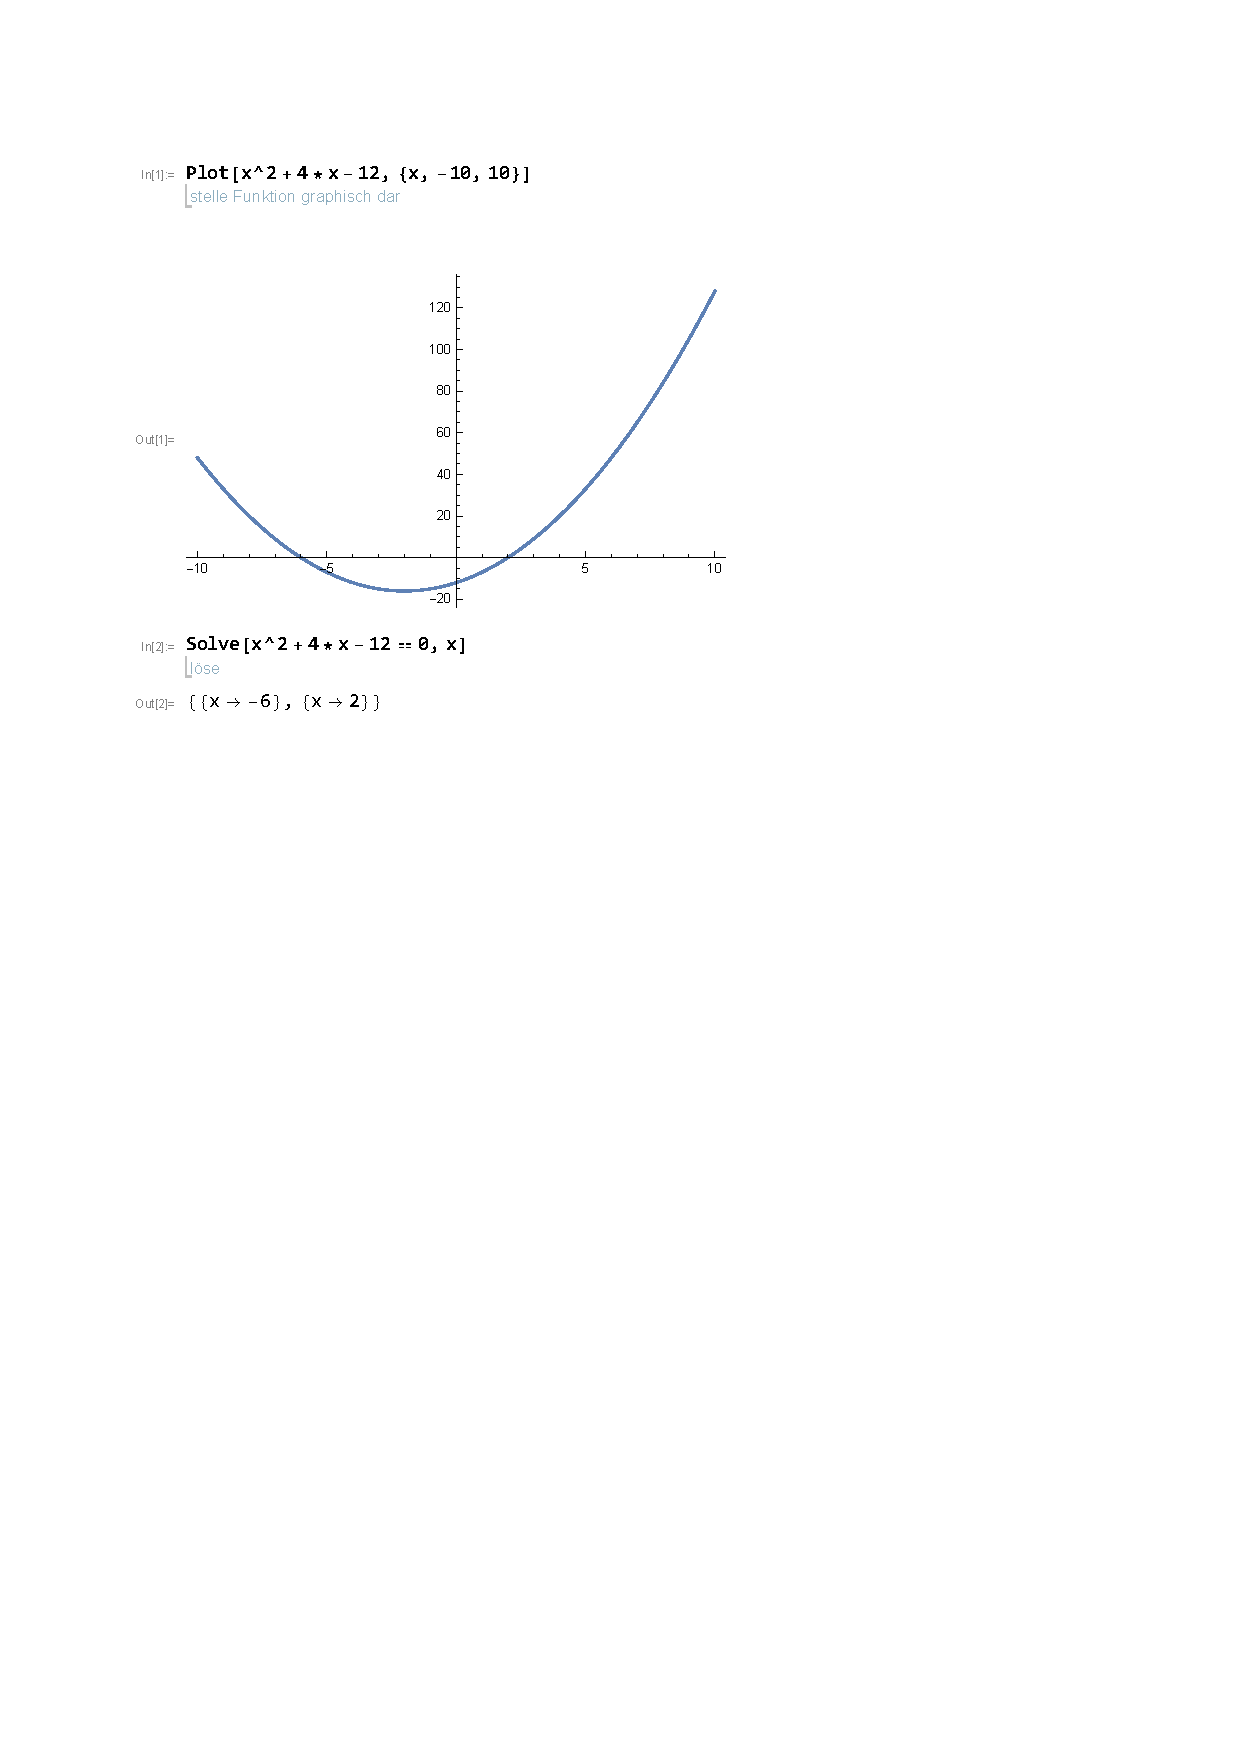
\includegraphics{./aufgabe_4.pdf}





 





\end{document}
